\documentclass{report}
\usepackage{graphicx}
\usepackage{fixlatvian}
\usepackage{verbatim}
\usepackage{circuitikz}
\usepackage{pgfplots}

\title{Vienkāršu elektrisku shēmu modelēšana}
\author{Edgars Voicišs}
\date{Marts 2018}

\begin{document}
\maketitle

\chapter{Teorētiskā daļa}
\section{Ķēdes aprēķins}

Apēķiniet spriegumus uz rezistoriem attēlā dotajā shēmā. Sprieguma avota V1 sprieguma vērtību U (Voltos) izvēlieties daļskaitli, kas būtu Jūsu apliecības pēdējie trīs cipari dalīti ar10. Piemēram. ‘101REB123’ nozīmē V1 = 12.3 (Volti), R1 ir apliecības pēdējo 3 ciparu otrais numurs+1, R2 ir apliecības numura pēdējais cipars +1.\cite{1.avots} Piemēram, ja Jūsu apliecības numurs ir ‘101REB123’ tad ‘R1=3’, ‘R2=4’. Nofotografējiet aprēķinu vai saglabājiet lapiņu. Aprēķina gaitabūs nepieciešama darbā ‘P02’. Turklāt, aprēķins būs jāpievieno atskaitei, ko veiksiet semestra beigās.\cite{2.avots} Piemērs 171REB083 V1 = 83/10=8.3 R1 = 8+1=9 R2 = 3+1=4.



\begin{table}[!b]
\centering
\begin{tabular}{|c|c|}
\hline
R1 & 9 \\
\hline
R2 & 4 \\
\hline
V1 & 8.3\\
\hline
UR1 & 5.7\\
\hline
UR2 & 6.2\\
\hline
\end{tabular}
\caption{Vērtību tabula}
\end{table}




\begin{center}
\end{center}
\begin{circuitikz}[american voltages]
\draw
   (0,4)to [V, l_=$Us$] (0,0)
   to [short, *-] (6,0)
   to (6,2)
   to [R, l_=$R$] (6,4)
   to [short, ] (5,4)
   to (3,4) to [open, ] (0,4)
   to [short, ] (1,4)
   to [R, l=$R$] (3,4)
   to (4,4)
\end{circuitikz}

\vspace{2cm}




\pgfplotsset{width=10cm,compat=1.9}
\begin{tikzpicture}
\begin{axis}
\addplot[color=red]{6.2==4};
\end{axis}
\end{tikzpicture}
UR2=f(R2)




\chapter{Praktiskā daļa}
\section{Darbs ar GEDA programmām}
\subsection{Darbs ar gschem}




\begin{figure}[!b]
\centering
\rotatebox{-90}{\includegraphics[width=7cm]{01.ps}}
\caption{Gschem elektriskā shēma}
\label{1}
\end{figure}

\subsection{Darbs ar gnetlist}
\verbatiminput{01.net}
\subsection{Darbs ar ngspice}




\begin{figure}[!h]
\centering
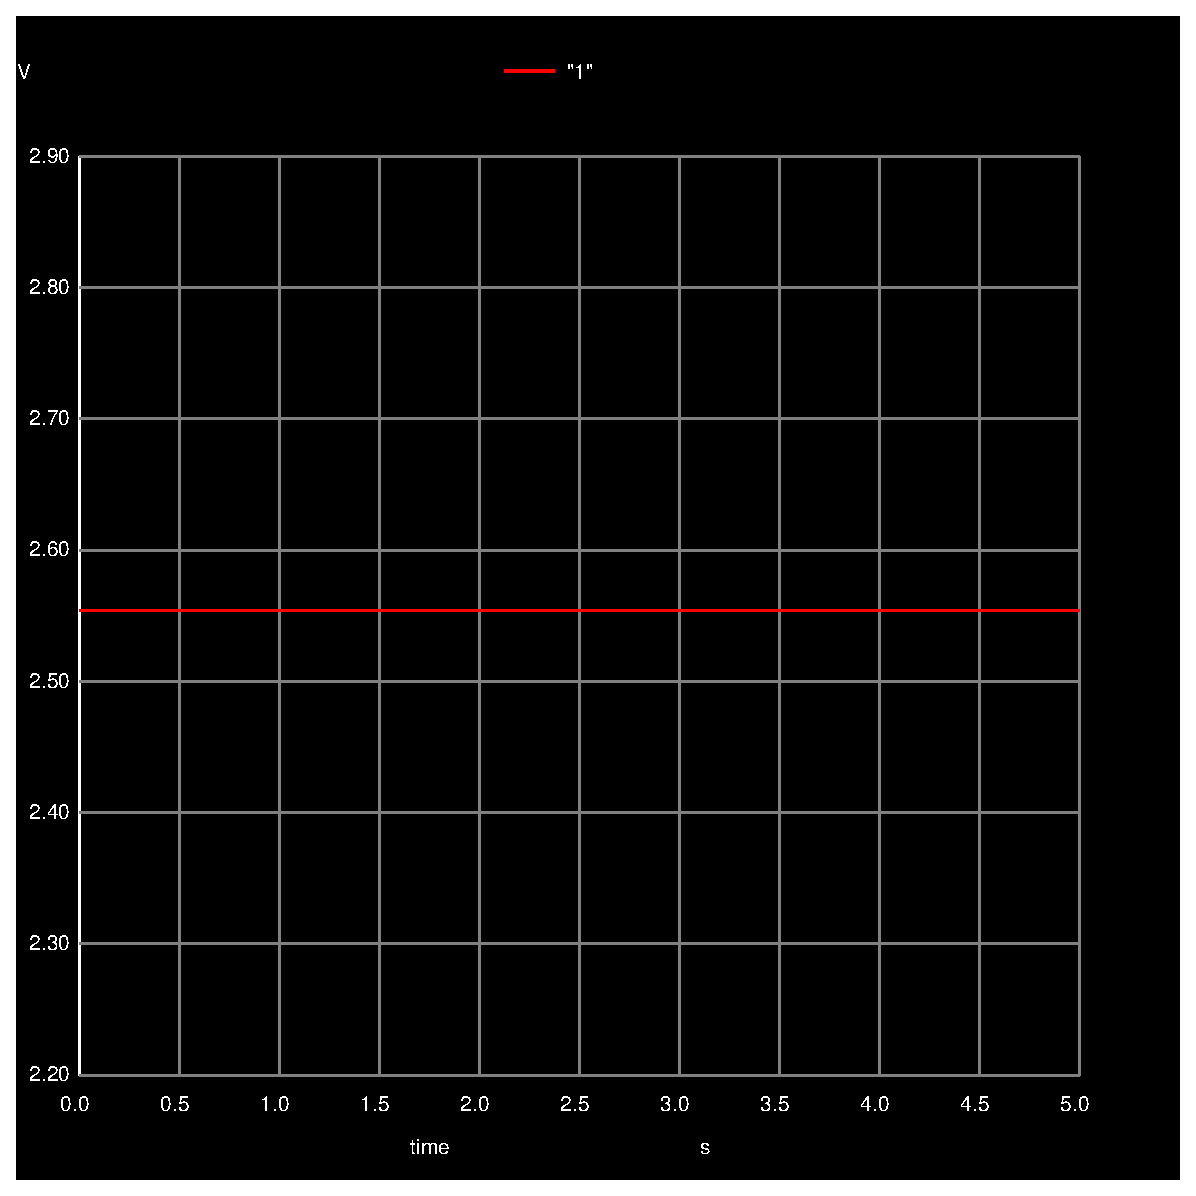
\includegraphics[width=5cm, height=5cm]{011.ps}
\caption{1.ngspice shēma}
\label{2}
\end{figure}
\begin{figure}
    \centering
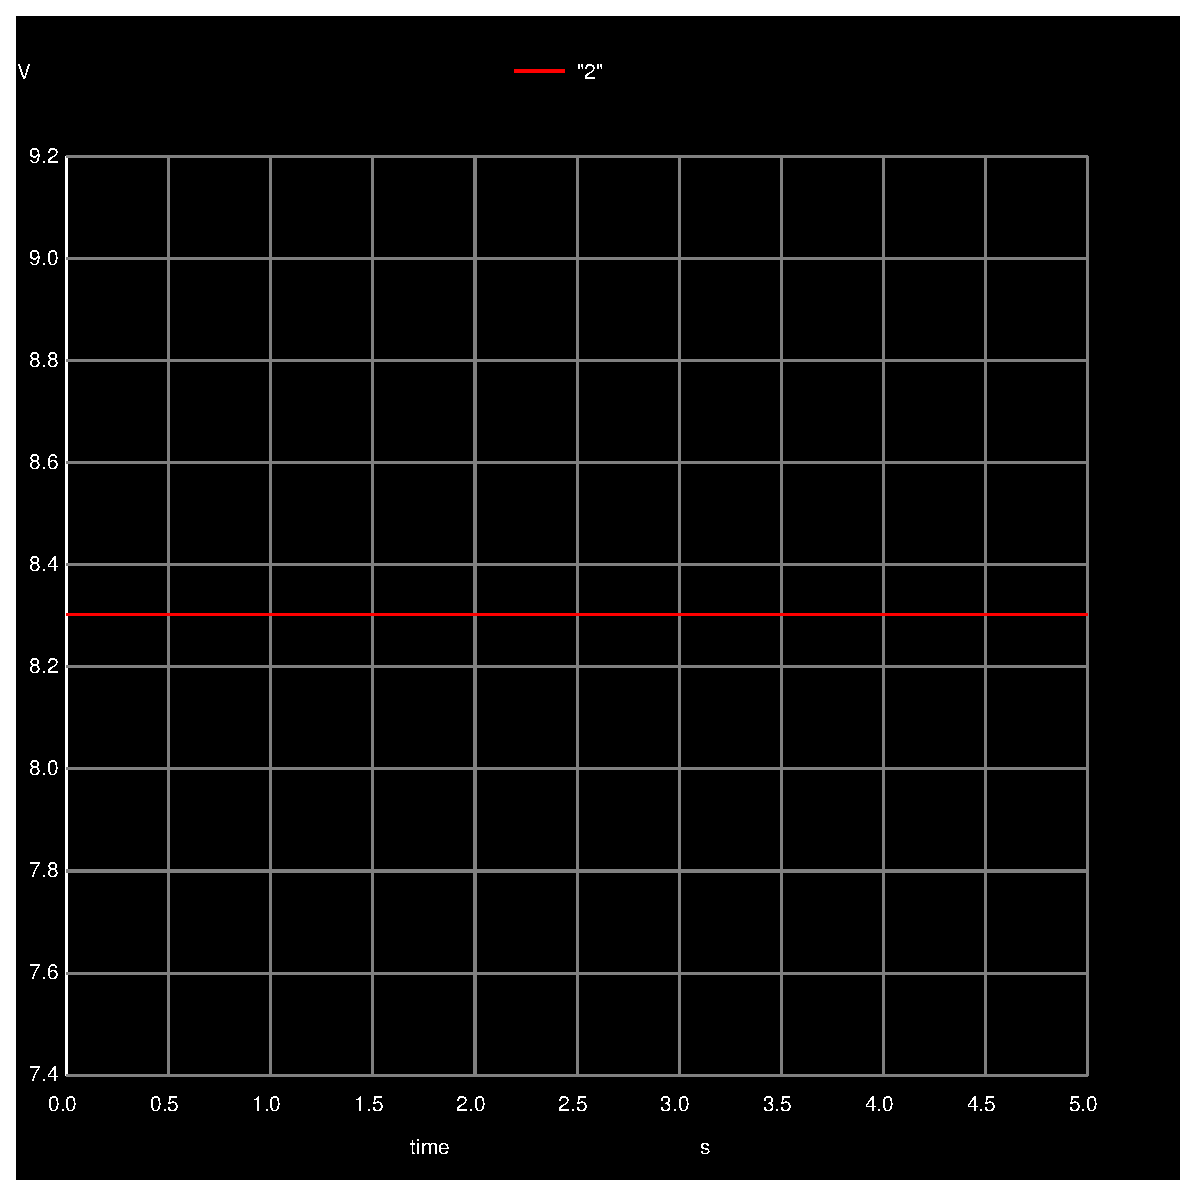
\includegraphics[width=5cm, height=5cm]{012.ps}
    \caption{2.ngspice shēma}
    \label{3}
\end{figure}




\vspace{6cm}
\section{Darbs ar QUCS programmām}
\begin{figure}[!h]
    \centering
\rotatebox{-90}{\includegraphics[trim={0 1cm 11cm 4cm},clip]{print.ps}}
    \caption{Darbs ar QUCS}
    \label{4}
\end{figure}




1. Simulācijas attēlošana ar Parameter sweep papildinājumu, kas palīdz viegli salikt nepieciešamos parametrus, ētrai simulācijas datu uzņemšanai.
2. Mērījumu tabula, un grafika līkne parāda izejas sprieguma vērtības atkarībā no R2 rezistora uzdotās vērtības x, veicot uzdoto simulāciju.




\begin{thebibliography}{9}
\bibitem{1.avots}
Albert Einstein. 
\textit{Zur Elektrodynamik bewegter K{\"o}rper}. (German) 
[\textit{On the electrodynamics of moving bodies}]
Annalen der Physik, 322(10):891–921, 1905.

\bibitem{2.avots} 
Michel Goossens, Frank Mittelbach, and Alexander Samarin. 
\textit{The \LaTeX\ Companion}. 
Addison-Wesley, Reading, Massachusetts, 1993.
\end{thebibliography}






\end{document}